% Preamble
\documentclass[a4paper,12pt]{article}

\usepackage[osf]{mathpazo} % palatino
\usepackage{ms}            % load the template
\usepackage[round]{natbib} % author-year citations
\usepackage{graphicx}
\usepackage{parskip} 
\usepackage{caption}
\usepackage{subcaption}
\usepackage{textcomp} % for parts per mille symbol     
\pagenumbering{arabic}    
\linespread{1.66}

% Title page information
\title{Reconstructing the last known movements of one of Nature's giants}
% 90 characters max

\author{
  Clive N. Trueman$^{1}$, Andrew L. Jackson$^{2}$, Katharyn S. Chadwick$^{1}$,\\ 
  Ellen J. Coombs$^{3,4}$, Sarah Magozzi$^{1,5}$, Richard C. Sabin$^{3}$ \\
  and Natalie Cooper$^{3*}$
}
\date{}
\affiliation{\noindent{\footnotesize
  $^1$ Ocean and Earth Science, University of Southampton Waterfront Campus, Southampton, SO14 3ZH, UK.\\
  $^2$ School of Natural Sciences, Trinity College Dublin, Dublin 2, Ireland.\\
  $^3$ Department of Life Sciences, Natural History Museum London, Cromwell Road, London, SW7 5BD, UK.\\ 
  $^4$ Department of Earth Sciences, University College London, Gower Street, London, WC1E 6BT, UK.\\
  $^5$ Department of Geology and Geophysics, University of Utah, Salt Lake City, UT 84112-0102, USA.\\
  $*$Email address: natalie.cooper@nhm.ac.uk
}}

\vfill

%\runninghead{}
%\keywords{}
%}

% End of preamble

\begin{document}
\modulolinenumbers[1]   % Line numbering on every line

\mstitlepage

\parindent = 1.5em
\addtolength{\parskip}{.9em}

\raggedright

\section{Abstract}

The spatial ecology of rare, migratory oceanic mammals such as blue
whales (\textit{Balaenoptera musculus}) is difficult to study directly. 
Recent advances in satellite telemetry have improved our understanding of individual-level migratory behavior, but tags generally last only a few months, and cannot provide retrospective information. 
Incrementally-grown tissues provide an alternative means of reconstructing individual-level movements over long timescales, but inferring spatio-temporal information from biochemical tracers is challenging. 
Here we present a new approach combining stable isotope analyses of incrementally-grown tissues with simulation models to infer individual-level animal movements. 
We use our new method to reconstruct multiple years of movement histories of individual modern and historic blue whales, including an iconic blue whale which stranded in 1891 and is now on display at the Natural History Museum, London.
Our method unlocks the information recorded in historic collections, and provides inferences that are complimentary to and comparable with tag-derived movement data.

\textbf{Keywords: carbon stable isotopes, movement models}

\section{Introduction}\label{background}

Migratory species pose a particular challenge for conservation practitioners because their effective conservation relies on protection at many, often distant, sites \citep{runge2014conserving}. 
Migratory species may also be particularly vulnerable to changes in climate or human use of the environment, as they are influenced by conditions in multiple locations across different parts of their life cycle \citep{robinson2009travelling}. 
Identifying threats to migratory species, understanding species responses to change and developing effective conservation measures all require information on the movements of individual animals over multiple years, ideally for both historic and present-day populations. 
With the development of electronic tagging technology, studies of the distributions of animals have largely shifted from infrequent observations of many individuals with limited or no information about individual movement behavior, to frequent observations of a few individuals, with detailed information about individual movement \citep{holdo2013inferring}. 
Despite the tremendous advances made using direct telemetry devices, tags are expensive, with a relatively high failure rate \citep{bailey2009behavioural,best2015tag,mate2007evolution}. 
Data on individual-level, multi-annual movements remain scarce, especially for rare, wide-ranging and long-lived marine species such as baleen whales (Mysticeti) \citep{ryan2013stable,hall2005stable,bailey2009behavioural}.

An alternative technique for investigating animal movements retrospectively is to use intrinsic biochemical information such as stable isotope compositions \citep{west2006stable,busquets2017estimating,hobson2008tracking}. 
Present-day populations can be studied with material collected in the field, while historic samples can be taken from museum collections; rich archives of behavioral information that are often under-utilised \citep{lister2011natural}. 
The stable isotope composition of animal tissues reflects the isotopic composition of diet at the time and place of ingestion, integrated over the timescale of tissue growth. 
A large literature describes the use of stable isotope markers to link the composition of a tissue to a geographic source at a single point in time \citep{hobson2008tracking}. 
Relating the isotopic compositions of marine animal tissues to the likely location of tissue growth is complicated by a lack of knowledge of spatial variations in the isotopic composition of diet (the isotopic baseline) \citep{west2006stable,mcmahon2015millennial}. 
This uncertainty is compounded when multiple samples are taken through time in the same individual, as temporal variation in the isotopic baseline must also be considered explicitly. 
Consequently, relatively little attention has been given to the potential to infer individual movement histories by reconstructing time series of multiple discrete origins from sequentially sampled incrementally-grown tissues.

Here we introduce a new approach to infer location from the isotopic compositions of sequentially-sampled incrementally-grown tissues by drawing on newly developed models predicting spatio-temporal variation in phytoplankton stable carbon isotope composition at global and monthly resolution \citep{magozzi2017using} (Fig. S3), coupled to an agent-based model of whale movements (see Supplementary Methods; Table S1; Fig. S5).
We use our coupled models to simulate time series of carbon stable isotope compositions expected under different movement behaviours. 
We then compare simulated isotopic profiles with the measured profiles to identify potential movement histories most consistent with the measured isotopic profile.

We apply our method to blue whales (\textit{Balaenoptera musculus}), the largest animal to have ever lived. 
Mysticete whales are characterized by the development of baleen, keratinous structures in the upper jaw used to filter food items from seawater. 
Baleen is ideal for stable isotope studies because keratin grows continuously through an individual's life, and once laid down it is metabolically inert \citep{best1996stable,hobson1998stable}. 
Baleen plates therefore offer a continuous isotopic record of behavior typically reflecting multiple years of life of an individual whale. 
Baleen is worn away at the tips over time, so a baleen plate reflects the most recent years of life, and rarely records an individual's entire lifespan. 
Among the mysticete whales, blue whales are a particularly attractive target for model-based isotope movement work as they have a consistent, low trophic level diet and feed continuously through the year, likely driven by high energetic costs of maintaining extreme muscle mass \citep{goldbogen2015}.

Similar to other large balaenopterid whales, blue whales are generally assumed to conduct annual migrations between high and low latitudes \citep{huckgaete2018}. 
As blue whales feed throughout the year to accommodate energetic costs, migration routes and feeding areas for blue whales are thought to be shaped by the year-round location of highly productive regions \citep{branch2007}. 
Recent studies tracking movements of individual blue whales primarily in the northeast Pacific have demonstrated high levels of among-individual variation in movement histories including suspending migration for opportunistic feeding and skipped migration (i.e. year round residency in either summer or winter
areas) \citep{busquets2017estimating}. 
The northeast Pacific population of blue whales is perhaps the best studied in terms of individual-level movements with a recent history of deployment of over 177 satellite tags \citep{irvine2017quantifying, mate2007evolution}.
In the northeast Pacific, satellite tags show individuals occupying most of the exclusive economic zone (EEZ) and into the Gulf of Alaska \citep{irvine2017quantifying} with greatest overlapping areas in the southern half of the EEZ, along the continental slope and shelf region between the California Channel Islands and Cape Mendocino. 
Winter feeding is less well characterized, but winter feeding grounds are known
in the Gulf of California and in the eastern tropical Pacific, specifically the Costa Rica Dome where production is maintained by seasonal upwelling.
However, most satellite deployments on blue whales report movement data for periods of time under six months \citep{heide2001new, silva2013north, bailey2009behavioural, lesage2017foraging, irvine2017quantifying}, and are unable to show individual movements between summer and winter feeding or breeding areas. 
The longest period of continuous monitoring via satellite tagging of an individual blue whale that we are aware of in the northeast Pacific is 504 days \citep{irvine2017quantifying} and in the North Atlantic is 177 days \citep{lesage2017foraging}.

The northeast Atlantic population of blue whales was the first large whale population to be systematically hunted with explosive harpoons, and while the population was probably relatively small before hunting, now around 1000 individuals are estimated to be in the northeast Atlantic in summer, mainly distributed around Iceland \citep{pike2009note}. 
The small population size and oceanic habit makes blue whale movements extremely hard to study. 
A combination of historic whaling data, observations, satellite tracks and acoustic monitoring suggests that blue whales in the northeast Atlantic also track regions of high production throughout the year, at least some whales wintering in the upwelling systems between Mauritania and the Cape Verde Islands \citep{baines2014upwellings}. 
Northward migration in the spring may occur along mid Atlantic corridors with peak sightings in the Azores around April-May \citep{silva2013north}. 
Summer feeding appears to occur in northerly latitudes around Iceland, and historically in the Norwegian and Barents Seas \citep{pike2009note}. 
Blue whales are frequently detected in waters to the west of the UK, with peak acoustic detections occurring between November and December, in southerly migrating animals \citep{reeves2004historical,baines2017autumn,charif2009acoustic,visser2011timing}.
To our knowledge one photographic identification has matched summer and winter locations of a single north-east Atlantic blue whale with sightings in Iceland and Mauritania \citep{poster}.

Inferences concerning movements of blue whales in general, and in the northeast Atlantic in particular, are therefore largely drawn from disparate information sources and rarely detail movements of individual animals over timescales of a year or more. 
It is particularly difficult to establish the degree of connectivity between summer and winter feeding areas, and the level of temporal consistency in movement behaviour within individuals. 
Information on historical movement patterns of individual blue whales is important for understanding the drivers of whale declines, and potential for human-whale conflicts as populations recover.

Here we infer individual level high-resolution movement records for seven blue whales for which baleen stable isotope data were available.
Isotope data for six whales stranding on the west coast of the USA or Mexico were reported in \cite{busquets2017estimating}, and we report new isotopic data from a whale stranding off the coast of Wexford Ireland in March 1891, and currently on display in the Natural History Museum, London (NHM).
The NHM whale ``Hope'' is a female estimated to be a young adult at least 15 years at death. 
Baleen from the NHM whale therefore yields information about migratory behaviors in North Atlantic blue whales around the peak of industrial whaling.

\section{Materials and Methods}\label{methods}

\subsection{Stable isotope extractions from baleen}\label{stable-isotope-extractions-from-baleen}

Baleen was collected from the Natural History Museum, London (specimen NHMUK.1892.3.1.1). 
The baleen plate was cleaned with ethanol to remove surface contaminants such as skin/gum or other lipids that can influence isotopic signals. 
{\raise.17ex\hbox{$\scriptstyle\sim$}}1mg samples of keratin powder were then collected from the plate using a hand-held drill and grinding bit. 
97 samples were taken at 1cm intervals, 0.5cm from the outer edge of the plate, starting at the proximal (gingival) section that contains the most recent tissue. 
Baleen grows at a constant rate, so the samples are equally spaced through time \citep{best1996stable}. 
Carbon and nitrogen isotope analysis was performed simultaneously via continuous-flow isotope ratio mass spectrometry at the University of Southampton SEAPORT Stable Isotope Ratio Mass Spectrometry Laboratory (Southampton, UK), using a Vario Isotope select elemental analyser, coupled to an Isoprime 100 isotope mass spectrometer. 
Replicates using internal laboratory standards (L-glutamic acid (C), Glutamic acid (CT standard), acetanilide and protein standard OAS) were used for quality control and calibration. 
C:N ratios for samples ranged from 3.28\text{\textperthousand} to 3.72\text{\textperthousand}, well within the acceptable theoretical range for pure keratin ($3.4\pm0.5$) allowing for comparison among samples \citep{hobson1998stable}. 
All data are available from the NHM Data Portal \citep{data-set} (https://doi.org/10.5519/0093278).

\subsection{Time calibrating stable isotope
profiles}\label{time-calibrating-stable-isotope-profiles}

Seasonal migrations across isotopic gradients induce cyclical variations in the isotopic composition of baleen, the distance between cycles reflecting growth rates \citep{hobson1998stable,busquets2017estimating}. 
Clear periodicity was evident in $\delta^{15}$N values across the entire baleen plate, and in $\delta^{13}$C values in the youngest 70 - 18cm of the plate (behavioural phase two). 
We calculated isotopic periodicity within the NHM baleen sample using Fourier Transform analysis \citep{cardona2017temporal} (Supplementary Figure S1), revealing a consistent growth rate of 13.5$cmy^{-1}$ which is remarkably similar to the mean isotope-derived baleen growth rates of $15.5 \pm 2.2cmy^{-1}$ estimated by \cite{busquets2017estimating}.  
Therefore we dated the youngest baleen sample as 1st March 1891, 24 days prior to the stranding date, 25th March 1891. 

\subsection{Baseline isotope
comparisons}\label{baseline-isotope-comparisons}

Isotope-enabled biogeochemical ocean models \citep{magozzi2017using,schmittner2016complementary} were used to characterize
the isotopic composition of phytoplankton expected in different
potential foraging grounds (Fig. S3). 
Annual average \(\delta^{15}\)N POM (particulate organic matter) values were provided by C.J. Somes (\textit{pers.comm}) based on a 5\({}^{\circ}\) resolution biogeochemical model (Fig. S3). \(\delta^{13}\)C POM values were simulated at 1\({}^{\circ}\) and monthly resolution using an isotopic extension to the NEMO-MEDUSA ocean biogeochemical model \citep{magozzi2017using,yool2013medusa}. 
Simulated \(\delta^{15}\)N POM values are relatively positive in the northeast Atlantic north of c. 60\({}^{\circ}\)N, and relatively negative in the central and southern North Atlantic. 
Annual average \(\delta^{13}\)C POM values largely vary with latitude, with more negative values in more northerly regions. 
In the central North Atlantic, \(\delta^{13}\)C POM values are relatively positive in the west, reflecting warm gulf stream waters (Fig. S3). 
The isotopic composition of carbon in phytoplankton also varies through seasons as isotopic fractionation of carbon during photosynthesis is strongly influenced by sea surface temperature \citep{magozzi2017using,laws1995dependence}. 
Thus temporal variations in \(\delta^{13}\)C POM values are superimposed on latitudinal gradients. 
The scale and nature of temporal variation in \(\delta^{13}\)C POM values also varies with latitude, with higher latitude seas showing greater intra-annual variation in \(\delta^{13}\)C POM values linked to strongly seasonal phytoplankton growth dynamics.
The model simulations used are forced with decadal climatological data from 2000-2010 \citep{magozzi2017using}. 
We do not draw inferences about location from absolute \(\delta^{13}\)C values and thus the reduction in oceanic \(\delta^{13}\)C POM values caused by release of fossil carbon into the atmosphere (Suess effect) does not influence inferences about location or movement. 
Ocean basin scale spatio-temporal differences in \(\delta^{13}\)C values largely reflect relative differences in sea surface temperatures between trophic, temperate and arctic waters, therefore we are confident that the \cite{magozzi2017using} model can be applied to interpret historic baleen isotope data.

We used \(\delta^{13}\)C POM values modeled at monthly resolution to simulate the isotopic expression of phytoplankton expected to be encountered by whales exhibiting differing movement behaviours. 
The stable isotope compositions of keratin at a given point in the baleen will reflect the stable isotope compositions of the krill it was feeding on in the weeks prior to keratin growth. 
Assimilation of carbon into krill tissues will dampen the temporal variability seen in POM, effectively producing a temporal average over the timescale of isotopic turnover within krill. 
We estimate turnover to be complete between two and four months and therefore we resampled the \(\delta^{13}\)C POM values in each one degree cell to reflect an average of isotopic compositions in phytoplankton in the two months prior to the sampling date. 
Average values were weighted according to the proportional plankton biomass estimated for each month. 
Carbon isotope values are also likely to be fractionated during transfer from plankton to krill as \textsuperscript{12}C is preferentially lost through respiration. 
The degree of such trophic fractionation is unclear, however and we do not draw interpretations based on absolute \(\delta^{13}\)C values, rather on the relative \(\delta^{13}\)C values across the length of the baleen plate. 
We assume opportunistic ingestion of protein throughout the year \citep{baines2017autumn,silva2013north,visser2011timing,busquets2017estimating, lesage2017foraging, bailey2009behavioural, branch2007, huckgaete2018}.

\subsection{Agent-based whale movement
model}\label{agent-based-whale-movement-model}

We simulated whale movements with the likelihood, direction, and extent of movement influenced by behavioral state, sea surface temperature, water depth, and phytoplankton concentration (as a proxy for zooplankton food availability).
Movement was coded as a set of probabilistic rules, informed by the literature on blue whale behavior (e.g. \citep{handbook}).
All terms were expressed as probability distributions, yielding multiple potential movement tracks.

In the models, the likelihood of movement, direction (north, south, east, west, northeast, northwest, southeast, or southwest) and linear distance of movement are all influenced by the following. 
(i) Behavioural state (migrating north, migrating south, or foraging).
Northerly migrations were possible only in spring, and southerly migrations in autumn. 
Foraging was possible at any time of year, and was triggered when whales encountered high concentrations of plankton.
(ii) Sea surface temperature \citep{yool2013medusa} ($^{\circ}$C). 
When migrating north, whales were more likely to move towards lower temperatures provided they were above the minimum temperature threshold (3$^{\circ}$C); whereas whales migrating south sought warmer waters.  
(iii) Water depth (m; from the General Bathymetric Chart of the Oceans (GEBCO) global bathymetry dataset\citep{bathy}, extracted via the marmap package in R \citep{marmap}). 
Whales were less likely to move into waters less than 400m deep, and increasingly unlikely to move into even shallower waters. 
(iv) Phytoplankton concentration ($mmolNm^{-3}$, for combined diatom and non-diatom communities \citep{yool2013medusa}). 
This was included as a proxy for zooplankton food availability. 
Whales are more likely to move towards (or remain within) areas of high phytoplankton density, particularly during the foraging behavioural state. 

For Pacific whales where satellite data offers a rich view of individual movements, we coded our movement models to reflect either residency in southern waters (between Baja California and the Costa Rica Dome) or seasonal latitudinal movements within the California current system. 
We simulated 250 movement tracks of four years duration. 
We allowed start and end dates to vary by aligning measured profiles to sections of simulated profiles of identical lengths with sequentially changing start dates and saved best fitting models.

For the historic North Atlantic whale, we simulated the isotopicexpression expected for (a) residency in each known hotspot for blue whale sightings or historic hunting grounds in the North Atlantic (Norwegian/Barents Sea, West Ireland, Canaries/Azores and Mid Atlantic Ridge, and the Cape Verde/Mauritanian upwelling area \citep{mcdonald2006biogeographic,reilly2008balaenoptera,sigurjonsson1995life}; Supplemental Figure S4); (b) seasonal migration between high sub-Arctic latitudes and temperate latitudes around the British Isles and (c) seasonal migration between high latitudes and subtropical latitudes.
Measured tracks can only be replicated by combination of residency and seasonal migration with latitudinal migrations limited to the last four
years of simulations. 
For a full description of the model and its parameters see Supplementary Methods: Fig. S5 and Table S1. 
We simulated seven years of whale movements 1000 times and two years of residency 30 times for each residency hotspot (Fig. S4).
We simulated whale movements 1200 times, then excluded simulations where the virtual whale stranded before reaching the 3019 days of the baleen record, leaving 1049 simulations.

At each time point and location in the simulations, we extracted time averaged \(\delta^{13}\)C values from the spatio-temporal model \citep{magozzi2017using} resulting in a range of simulated isotopic profiles for different migration patterns and foraging areas (Figs X, \ref{fig2}, and S4).
We then compared the simulated stable isotope profiles (Figure \ref{fig3}) to the profile of the blue whale (Figure \ref{fig1}).

R code for all analyses is available from GitHub (https://github.com/nhcooper123/blue-whale-bes; \citep{github})

\section{Results and Discussion}

\subsection{Matching model to Pacific data.}

Estimates of baleen growth rates for the six modern whales from the northeast Pacific were inferred from cyclical fluctuations in nitrogen isotope ratios and reported in \cite{busquets2017estimating}. 
We used these growth rates to reconstruct a potential timeline for baleen isotope records.

% Pacific whales figure
\begin{figure}
 \centering
  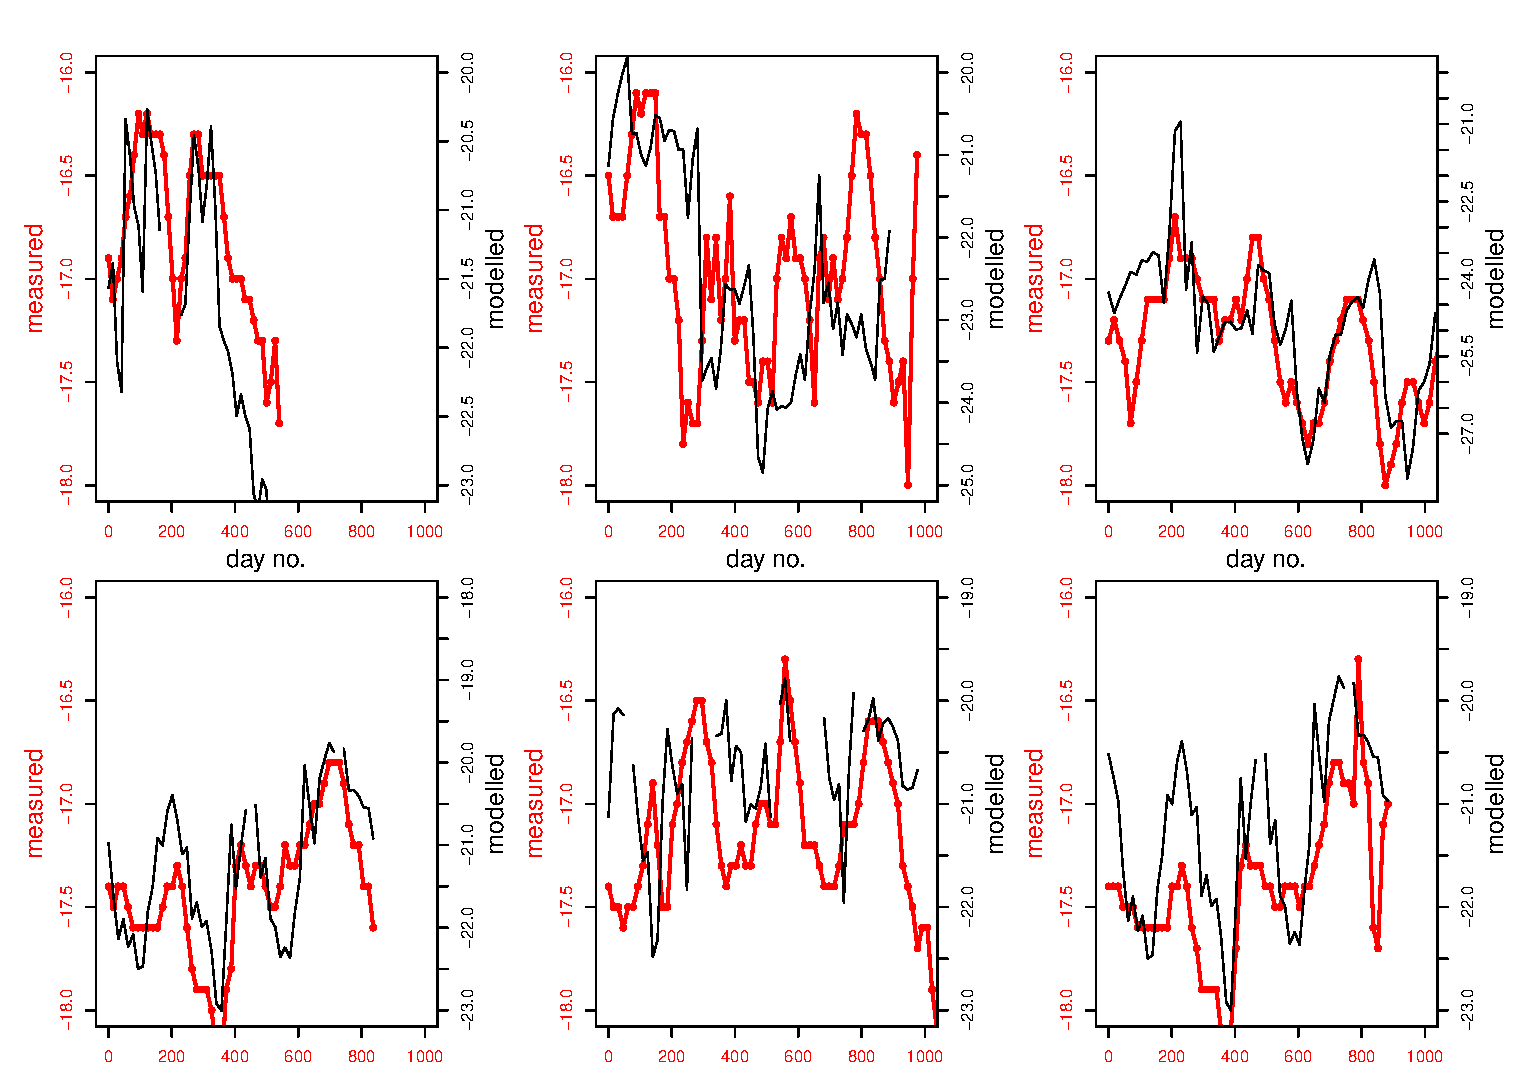
\includegraphics[width = \linewidth]{figures/figure-Pacific-draft.eps}
  \caption{Correlations among simulated $\delta^{13}$C from the best fitting migratory movement models (grey lines, right hand y-axis) and $\delta^{13}$C from baleen (black line, left hand y-axis) for six Pacific blue whales taken from \cite{busquets2017estimating}. 
  Simulated $\delta^{13}$C values are six month moving average values for the time series of simulated plankton $\delta^{13}$C values in that location, reflecting temporal integration of phytoplankton $\delta^{13}$C values within the food chain before ingestion by the whale as krill. 
  The end points of the simulations and empirical data have been aligned to coincide.
}
  \label{pacific}
\end{figure}

In four of the six cases, measured baleen carbon isotope profiles could be replicated from model simulations with relatively high precision (Fig. \ref{pacific}
; best fit r\textsuperscript{2} values ranging from 0.43 to 0.74).
Whales D and F showed similar carbon isotope records and were best fit by the same movement simulation. 
We extracted monthly locations associated with the best fitting simulation models for each whale (Fig. \ref{pacific}).
Best fitting simulation models for whales D and F imply a relatively southerly distribution with few locations north of Baja, California and relatively limited seasonal latitudinal migration. 
The measured carbon isotope record for whale A was best fitted by simulations with a southerly distribution, but with an additional strong seasonal latitudinal migration, and with more northerly locations between April and October. 
Whale C was best fit by models with relatively northerly locations and strong seasonal latitudinal migration. 
We were unable to find convincing fits to baleen profiles for whales B and E suggesting that longer simulations with a greater variation in movements were needed. 
The inferred movement records are consistent with the known spatial distributions and relatively high level of individual variation in spatial distributions among blue whales in the Pacific northwest \citep{irvine2017quantifying, mate2007evolution}.

\subsection{Atlantic whale baleen measured isotopic record}

For Hope, the historic North Atlantic whale, \(\delta^{15}\)N values record regular cyclical fluctuations throughout the length of the baleen plate, with a mean spacing of 13.5cm, assumed to represent annual periodicity (see Supplementary Methods). 
Therefore, given the date of stranding (25th March 1891), and estimated baleen growth rates of 13.5cm\(y^{- 1}\), we reconstructed a timeline for \(\delta^{13}\)C and \(\delta^{15}\)N fluctuations in the baleen over seven full years of the whale's life (early 1884 - spring 1891). 
The \(\delta^{13}\)C and \(\delta^{15}\)N profiles show two distinct phases in the whale's behaviour. 
In behavioural phase one (from the start of the record to spring 1886), we find relatively stable, elevated \(\delta^{13}\)C values, and relatively low \(\delta^{15}\)N values (Fig. \ref{fig1}; Figs. S1 and S2). 
In behavioural phase two (summer 1886 to spring 1890) \(\delta^{15}\)N values are relatively elevated and \(\delta^{13}\)C values are relatively depleted with coincident cyclical fluctuations in both \(\delta^{13}\)C and \(\delta^{15}\)N values. 
In the last year of life the cyclical pattern is disrupted, with constant low \(\delta^{13}\)C values for approximately six months in the first half of 1890, before a rapid switch to relatively positive \(\delta^{13}\)C values in the second half of 1890. 
The final three months of the record show a progressive fall in \(\delta^{13}\)C values (Fig. \ref{fig1}; Figs. S1 and S2).

% figure 1
\begin{figure}
  \centering
  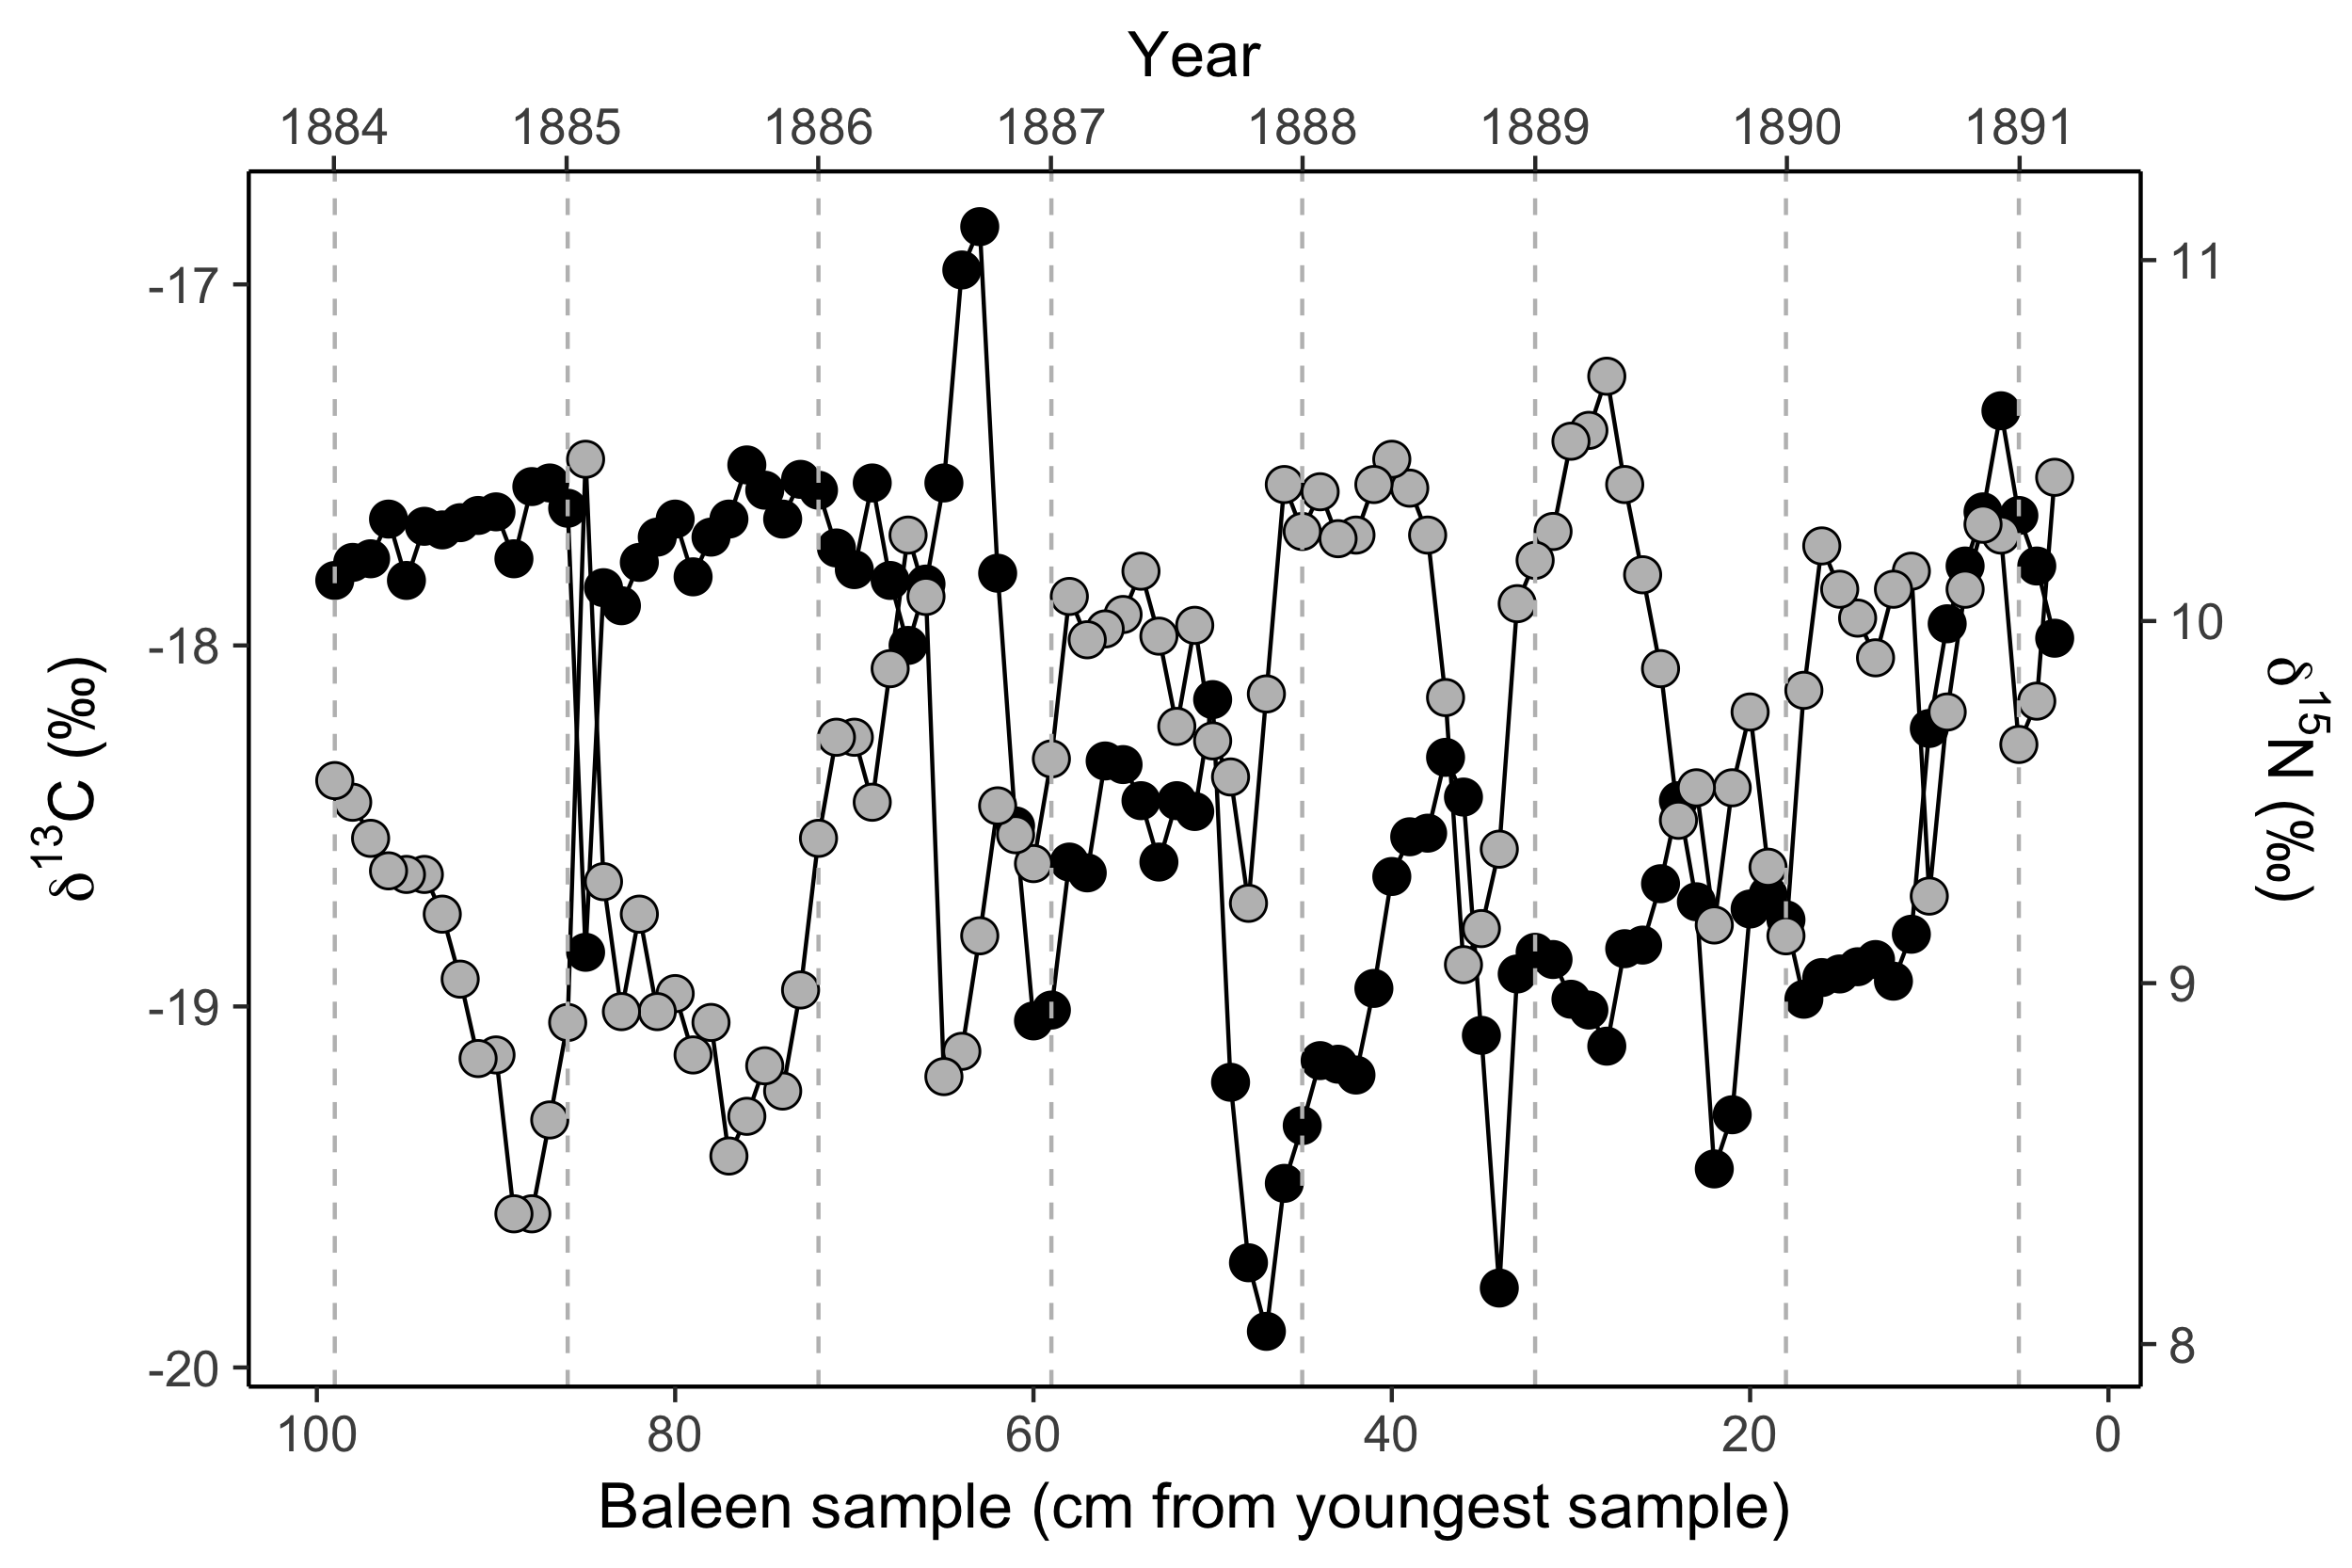
\includegraphics[width = \linewidth]{figures/Figure-1-raw-dC-dN-data.png}
  \caption{Variation in stable isotope values in the NHM blue whale, expressed as $\delta^{13}$C (black circles, left y-axis) and $\delta^{15}$N (grey circles, right y-axis). Samples were taken longitudinally through the baleen plate (n = 97 samples from a single baleen plate for both isotopes). There is strong annual periodicity and cross-correlation (Supplemental Figures S1 and S2) in both isotopes. The approximate relationship to years assuming a growth rate of 13.5cm y$^{-1}$ is shown on the upper x-axis, and year boundaries are indicated by vertical dotted grey lines.}
  \label{fig1}
\end{figure}

% figure 2
\begin{figure}
 \centering
 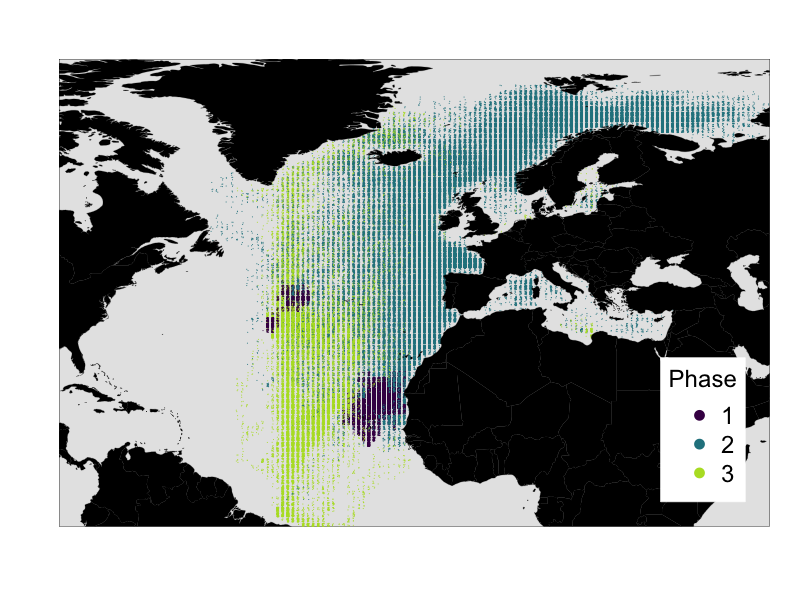
\includegraphics[width = \linewidth]{figures/Figure-2-points.png}
  \caption{Simulated locations of the whale taken from the top 10\% best fitting migratory movement models. 
  Colours reflect the behavioural phase. 
  Phase one is early 1884 to spring 1886, phase two is summer 1886 to spring 1890, and phase three is spring 1890 to spring 1891.}
  \label{fig2}
\end{figure}

The relatively positive and seasonally-invariant \(\delta^{13}\)C values seen during behavioural phase one are only found in subtropical areas of the North Atlantic. 
Our simulations identify a range of possible locations for the whale (Fig. \ref{fig3}), although areas around the Mauritanian coast and Cape Verde Islands, a known current and historic winter feeding area for blue whales \citep{baines2014upwellings,reeves2004historical}, and potentially to the west of the Azores (Figure \ref{fig2}), most closely match the measured profile. 
The whale remained in these warm waters for at least one full year. 
Hope was estimated to be at least 15 years old when she died (based on vertebral epiphyseal fusion; R.C. Sabin \textit{pers.comm}), so was probably older than 10 years old, and therefore sexually mature, during this period. 
During behavioral phase two, the observed low \(\delta^{13}\)C values imply foraging in colder, more northerly latitudes. 
The pronounced cyclical variations in \(\delta^{13}\)C values observed during behavioral phase two could reflect either the isotopic expression of the spring phytoplankton bloom in northern waters \citep{magozzi2017using}, latitudinal migrations, or a combination of both.

% figure 3
\begin{figure}
 \centering
  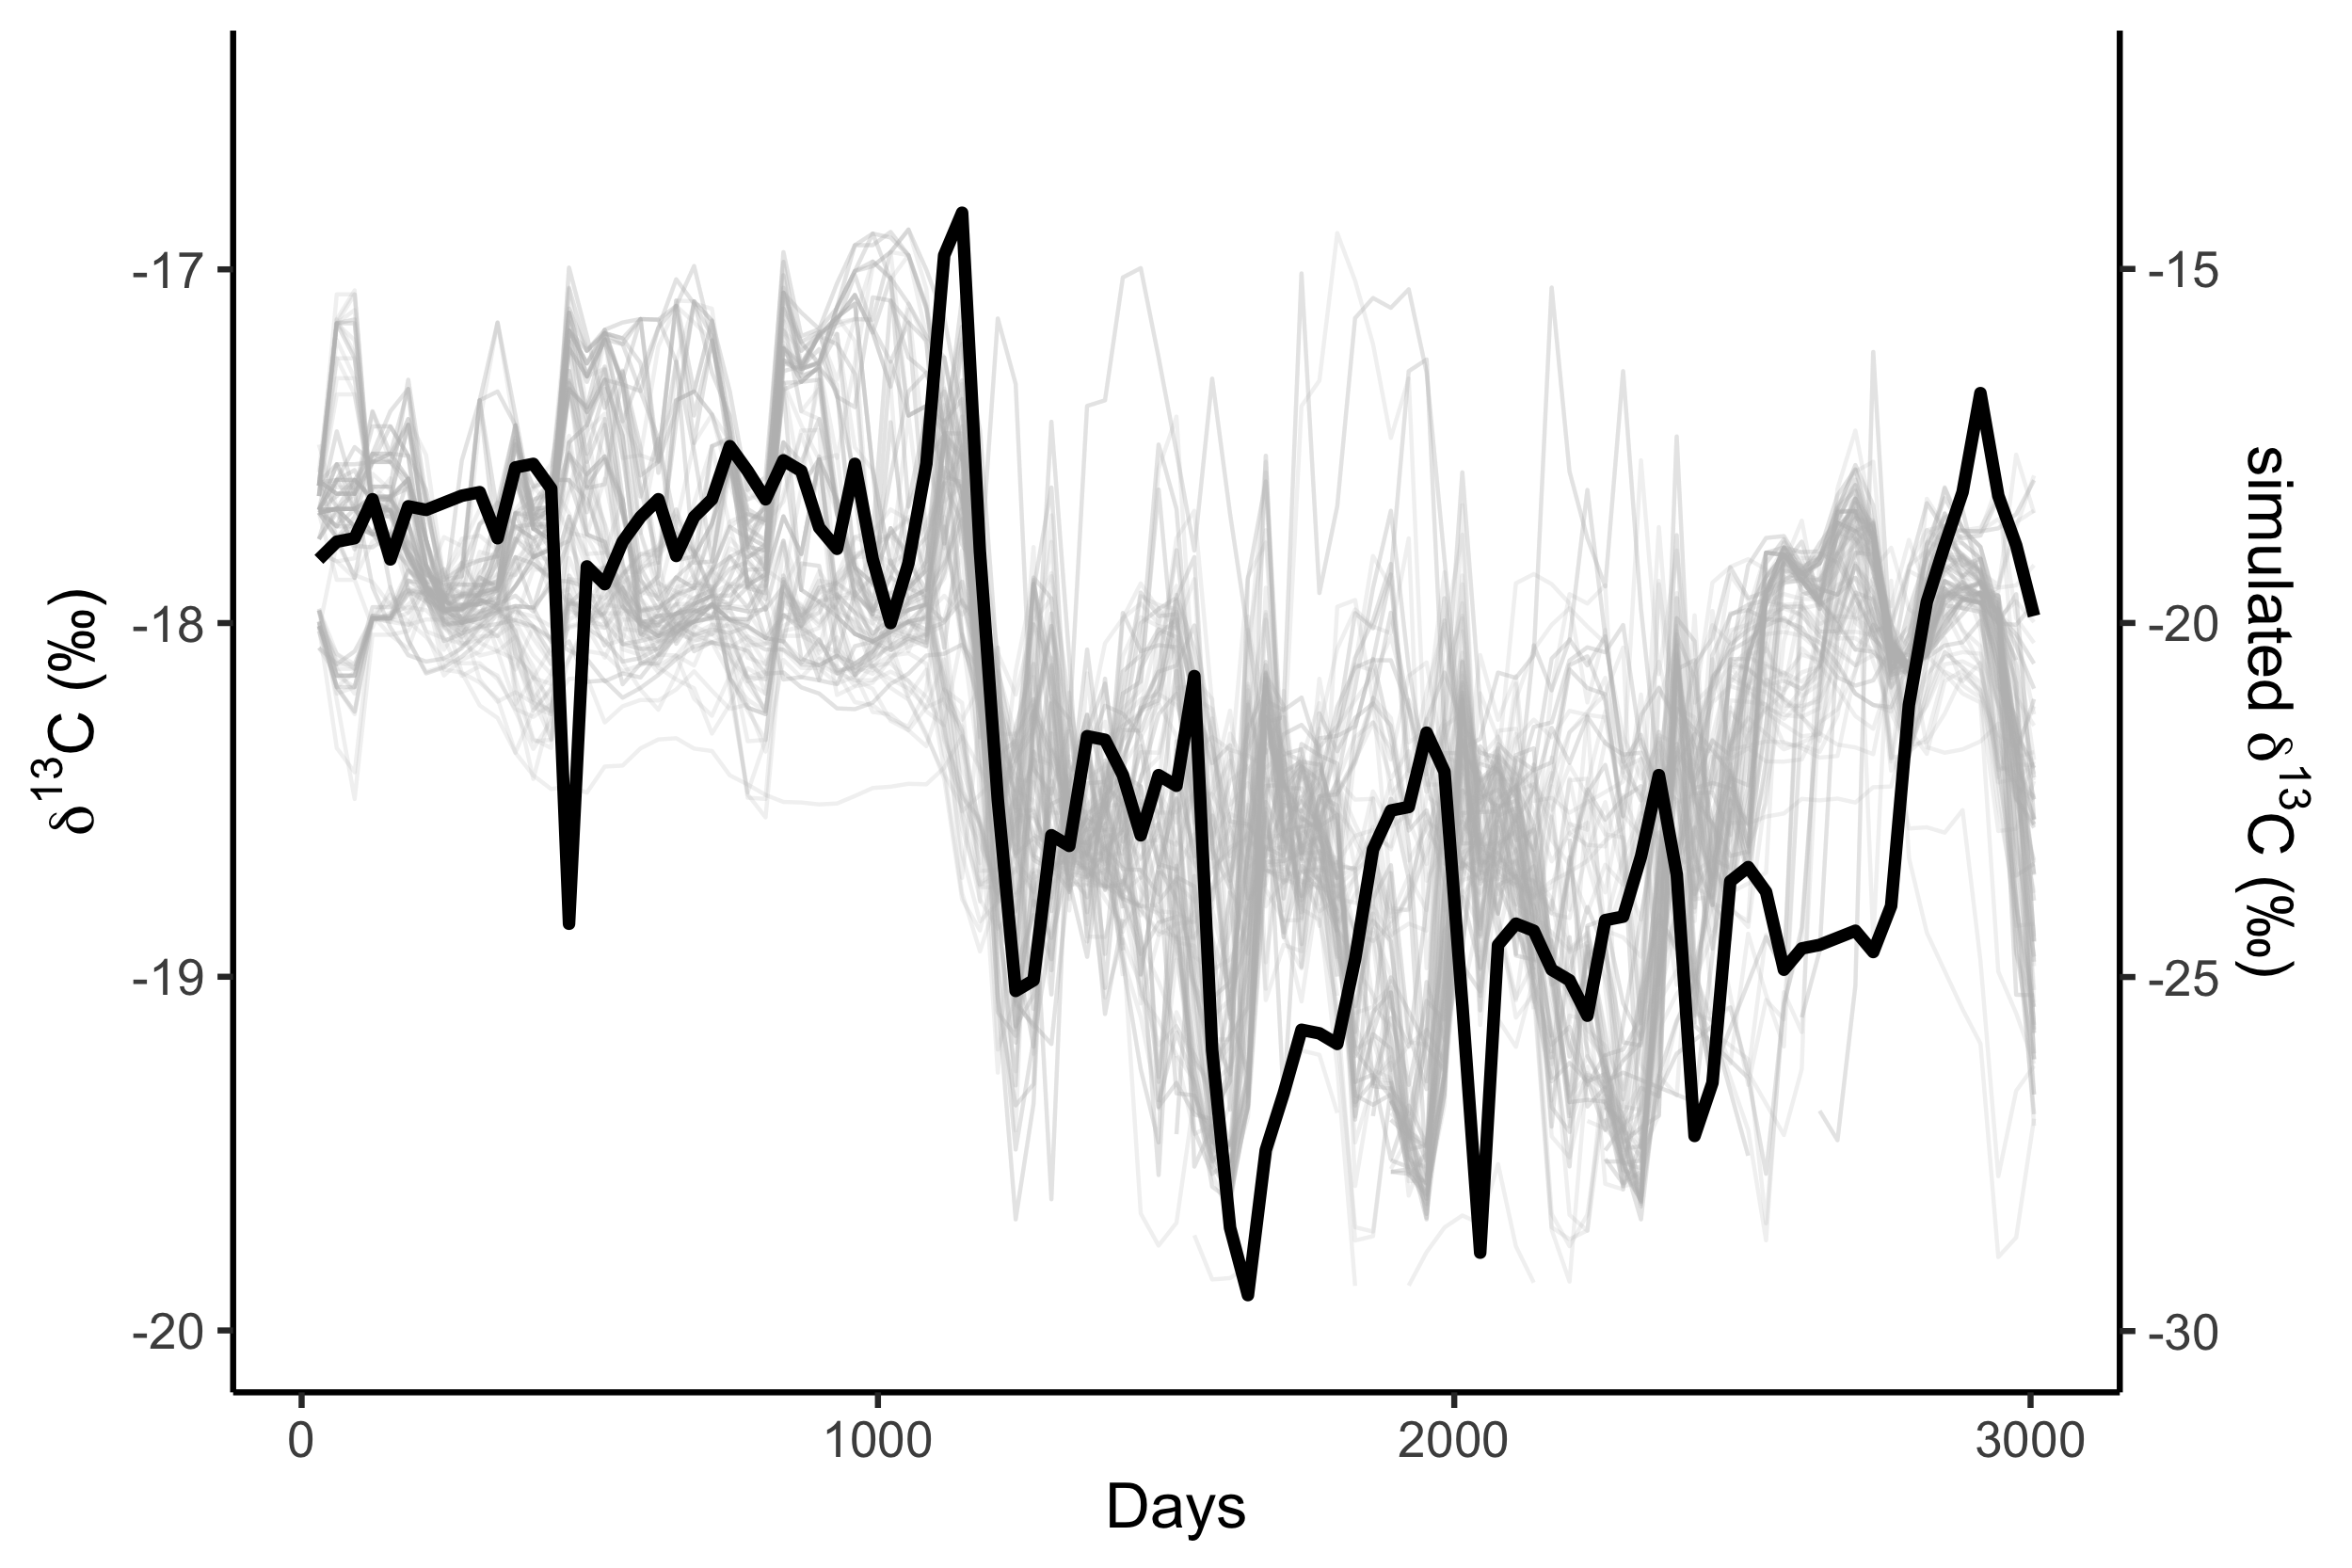
\includegraphics[width = \linewidth]{figures/Figure-3-blue-sims.png}
  \caption{Correlations among simulated $\delta^{13}$C from the top 10\% best fitting migratory movement models (grey lines, right hand y-axis) and $\delta^{13}$C from baleen (black line, left hand y-axis; see Figure \ref{fig1}). 
  Simulated $\delta^{13}$C values are six month moving average values for the time series of simulated plankton $\delta^{13}$C values in that location, reflecting temporal integration of phytoplankton $\delta^{13}$C values within the food chain before ingestion by the whale as krill. 
  The end points of the simulations and empirical data have been aligned to coincide.
}
  \label{fig3}
\end{figure}

We simulated 1200 individual movement patterns, then excluded simulations where the virtual whale stranded before reaching the 3019 days represented in the baleen.
We then compared the remaining 1049 simulations and the resulting simulated baleen $\delta^{13}$C records, to the measured records with simple linear regressions. 
Simulated baleen \(\delta^{13}\)C profiles produce a good fit to measured profiles, the median \(r^{2}\) value across 1049 simulated profiles was 0.31, and the maximum was 0.65 (Fig. S6). 
The top 10\% best fitting simulated profiles are shown in Fig. \ref{fig2}. 
Best fitting models predict residency in the Cape Verde region in behavioral phase one. 
Behavioral phase two is best simulated by seasonal migrations between summer foraging in northern areas (e.g. Norwegian Sea/Barents Sea/Iceland region), and winter foraging in a broad region between the UK and more southerly, subtropical waters. 
Better-fitting models in general were those predicting a greater latitudinal foraging range, and foraging in more northerly waters (Fig. S7 and S8). 
Best-fit model distributions are largely consistent with current understanding of blue whale distributions in the northeast Atlantic \citep{reeves2004historical,baines2014upwellings,baines2017autumn,reeves2004historical} with perhaps greater importance of winter foraging in temperate regions (Fig. \ref{fig4}).

% figure 4
\begin{figure}
 \centering
  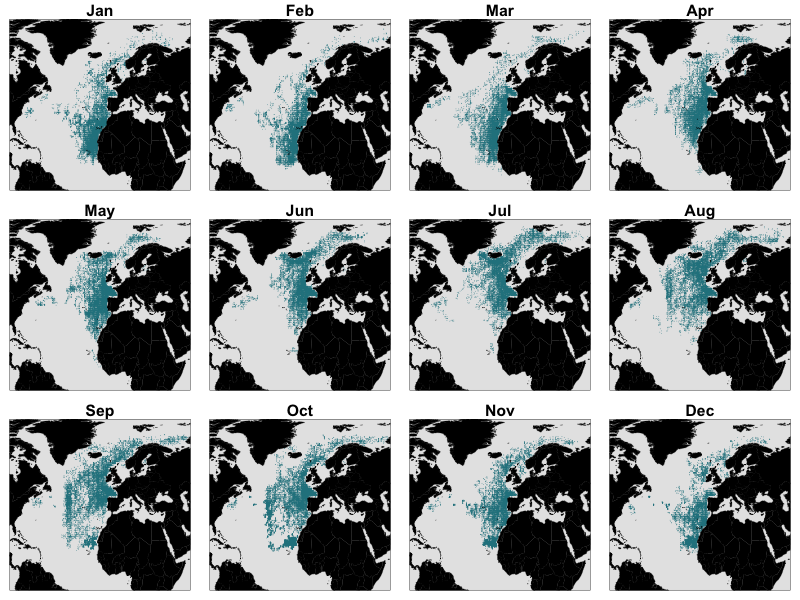
\includegraphics[width = \linewidth]{figures/Figure-4-monthly.png}
  \caption{Simulated locations by month taken from the top 10\% best fitting migratory movement models for behavioural phase two (summer 1886 to spring 1890) only.}
  \label{fig4}
\end{figure}

The last 500 days of Hope's life are difficult to simulate.
Beginning in the winter of 1889/1890, the observed \(\delta^{13}\)C values are relatively low, and remain constant for c.4-6 months, before increasing rapidly in the second half of 1890. 
Low \(\delta^{13}\)C values are found in northern waters, but these areas also show large temporal fluctuations in \(\delta^{13}\)C\textsubscript{plk} values (Fig. S4), and the observed values cannot be simulated purely from movements within the known geographic range. 
We suggest that the \(\delta^{13}\)C record in the last period of life may be associated with pregnancy and calf rearing. 
Constant, low \(\delta^{13}\)C values may reflect later metabolic release of carbon reserves assimilated from northern latitudes (i.e. a period of time with limited opportunistic foraging). 
After c.4-6 months the whale began ingesting food with relatively high \(\delta^{13}\)C values, indicating feeding in low latitude waters, shortly followed by a final northward migration. Blue whales have a 10-12 month gestation period, with calving occurring in subtropical waters, and calves are weaned after 6-7 months \citep{handbook}.
We therefore infer a movement chronology reflecting three years of uninterrupted annual latitudinal migrations leading to pregnancy in the
year 1889 and birth in the winter of 1889/1890. 
Following birth, we infer a period of c.4-6 months of residency in sub-tropical waters where the whale was sustained largely from stored lipid reserves, which we interpret as reflecting weaning. 
Subsequently we propose that the whale had a short period of feeding in sub-tropical waters in the second half of 1890 potentially during a final northward migration and eventual stranding during the return to northern feeding grounds in early 1891.

Whaling was an intense pressure for blue whales during the period we are
analysing. 
Before whaling in the North Atlantic began in 1868 \citep{reilly2008balaenoptera}, there were and estimated 10,000-15,000 blue whales in the region \citep{sigurjonsson1995life}. 
In the early 20th century, fisheries moved outside the area because stocks were so depleted \citep{reilly2008balaenoptera}; during this period over 12,000 blue whales were landed \citep{sigurjonsson1995life}. 
The NHM blue whale was thus an individual from a species at the brink of local extinction, potentially representing more than 0.1\% of the entire population of blue whales in the northeast Atlantic.
Inferring spatio-temporal distributions of populations from high density observations of a few individuals (or, in this case one individual) will always be problematic, but the predictive power linking a tracked individual to the population distribution increases when the tracked animal has a strong preference for specific habitats and there is a patchy (clumped) distribution of those habitats \citep{holdo2013inferring}. 
In the case of blue whales, the primary driver influencing seasonal movements is assumed to be the seasonally variable distribution of food resources between high and low latitudes. 
As blue whales have a relatively restricted diet that shows highly predictable spatio-temporal differences in abundance at least on ocean basin scales, we argue that the seasonal latitudinal migrations inferred during behavioural phase two are likely to be common movement traits within North Atlantic blue whales. 
This inference of course requires testing with additional isotopic records from individual whales, observational sightings data and multi-year satellite tracking records.

Our movement models suggest that the upwelling regions around Mauritania and the Cape Verde Islands may have been important historic calving areas, consistent with modern observations of juvenile blue whales in the northeast Atlantic \citep{handbook}.
These areas are now fishing, tourist and shipping hotspots with emerging offshore oil and gas exploration, potentially increasing threats to the recovery of the small population of blue whales in the northeast Atlantic. 
Although hunting for blue whales has been banned for over 50 years, the species is still listed as Endangered on the IUCN Red List, and expected recoveries following the cessation of active hunting may be impeded by other human activities such as modifications to the food web or more direct impacts of noise and shipping.
Developing an understanding of the nature and plasticity of individual level movements in populations of blue (and other mysticete) whales would aid management decision making in the conservation of this endangered species \citep{irvine2017quantifying}.

Long-term, multi-annual data on the movement patterns and reproductive ecology of individual blue whales are scarce. 
Although based on a few individuals, our results confirm that sequential sampling of stable isotope compositions in whale baleen, combined with simulation modeling can yield plausible inferences of individual whale movements that are consistent with population-level satellite tag data and/or inferences drawn from seasonal differences in distributions inferred from observations of multiple individuals over time and space. 
Our movement simulation modeling removes a long-standing limitation in stable isotope ecology, and can be applied to stable isotope records from any incrementally-grown tissue to estimate most likely individual movement behaviors over multiple years. 
By unlocking information contained in incrementally-grown tissues we hope that a more detailed picture of individual movement behaviour in modern and historic mysticete whales (and other animals) can be developed.

\section{Acknowledgments}\label{acknowledgments}
This work was funded by the British Ecological Society (grant: 5771/6815). 
We thank C.J. Somes for providing  $\delta^{15}$N POM data, Bastian Hambach and Megan Spencer at the University of Southampton SEAPORT isotope laboratory for assistance with stable isotope analyses, and Andrew Yool for allowing us to use and share NEMO-MEDUSA outputs.

% References
\bibliographystyle{refs}
%\bibliographystyle{authordate1}
\bibliography{blue-whale-abbreviations}

\subsection{Data Code and Materials}\label{data-code-and-materials}
Data are available from the NHM Data Portal (https://doi.org/10.5519/0093278). 
R code is available from GitHub (https://github.com/nhcooper123/blue-whale-bes)(Zenodo DOI 10.5281/zenodo.2542777).

\end{document}
